% Name: Matrix with highlighted blocks
% Description: A 4×4 matrix split into four 2×2 blocks, each shaded and named.
% Tags: block matrix, partition, highlight

\usetikzlibrary{matrix, fit, backgrounds}

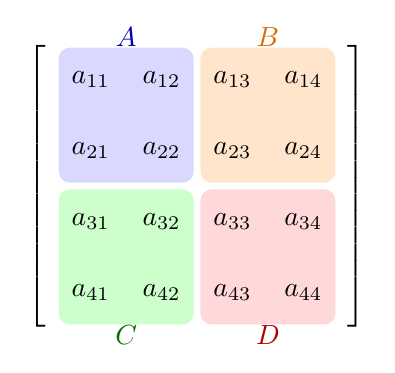
\begin{tikzpicture}
  \matrix (m) [
    matrix of math nodes, left delimiter={[}, right delimiter={]},
    nodes={minimum size=8mm}, column sep=1mm, row sep=1mm,
  ] {
    a_{11} & a_{12} & a_{13} & a_{14} \\
    a_{21} & a_{22} & a_{23} & a_{24} \\
    a_{31} & a_{32} & a_{33} & a_{34} \\
    a_{41} & a_{42} & a_{43} & a_{44} \\
  };
  \begin{scope}[on background layer, every node/.style={rounded corners, inner sep=0pt}]
    \node[fill=blue!15, fit=(m-1-1)(m-2-2), label={[blue!70!black]above:$A$}] {};
    \node[fill=orange!20, fit=(m-1-3)(m-2-4), label={[orange!85!black]above:$B$}] {};
    \node[fill=green!20, fit=(m-3-1)(m-4-2), label={[green!45!black]below:$C$}] {};
    \node[fill=red!15, fit=(m-3-3)(m-4-4), label={[red!70!black]below:$D$}] {};
  \end{scope}
\end{tikzpicture}
